%% ----------------------------------------------------------------------
\chapter{An M-dwarf candidate: L 279-94 (TIC 100796276)}
\label{ch:l27994}

L~279-94 is a nearby M dwarf (43.5~pc, $V = 13.9$, $T_\mathrm{mag} =
11.7$, declination $-53^\circ$) with a transit candidate reported by
P.~Rabtsevich in \emph{An 18-Day Planet Candidate around the Nearby Red
Dwarf L~279-94} (Zenodo, draft of 20~October 2026): an 18.152-day period,
a depth of 0.32~\%, a duration of 2.4~h and six TESS transits between 2020
and 2026, two of them predicted before the data were inspected. The note
is careful: it calls the signal a planet \emph{candidate}, because a
planet around a hidden companion star is still possible. Candidates around M dwarfs are
attractive because a small star makes a small planet easy to see, and
because their habitable zones lie at short periods. This chapter shows what
the pipeline concludes: why the candidate is not validated with the default
companion prior even though nothing argues against it, how it passes once
Gaia is used to limit the possible companions (MOLUSC), what that pass rests
on, and which observations would settle it.\footnote{Results of the runs of
6~November (pipeline v4.1.1), 19~November (v4.3, two identical runs, 10-min
bins) and 20~November 2026 (v4.3, 5-min bins; and 10-min bins with the
MOLUSC companions), all with TRICERATOPS+.}

\section*{Set-up}
The profile \code{profile_TIC100796276.json} gives the published ephemeris
(P = 18.15219~d, T0 = BTJD~2036.9763, 3200~ppm, 2.4~h) with a search of
$\pm3$~h around each predicted transit, the limb-darkened fit, the
neighbour vetting and the sensitivity test. TESS observed the star in five
sectors (27, 67, 94, 104, 105; full-frame images of 10 and 3.3~min). The
optimal apertures of 8--12 pixels hold 98.5--99.0~\% of the target's light;
the brightest neighbour within 2$'$ is 5.4~mag fainter
(Figure~\ref{fig:l279-field}).

\begin{figure}[ht]
\centering
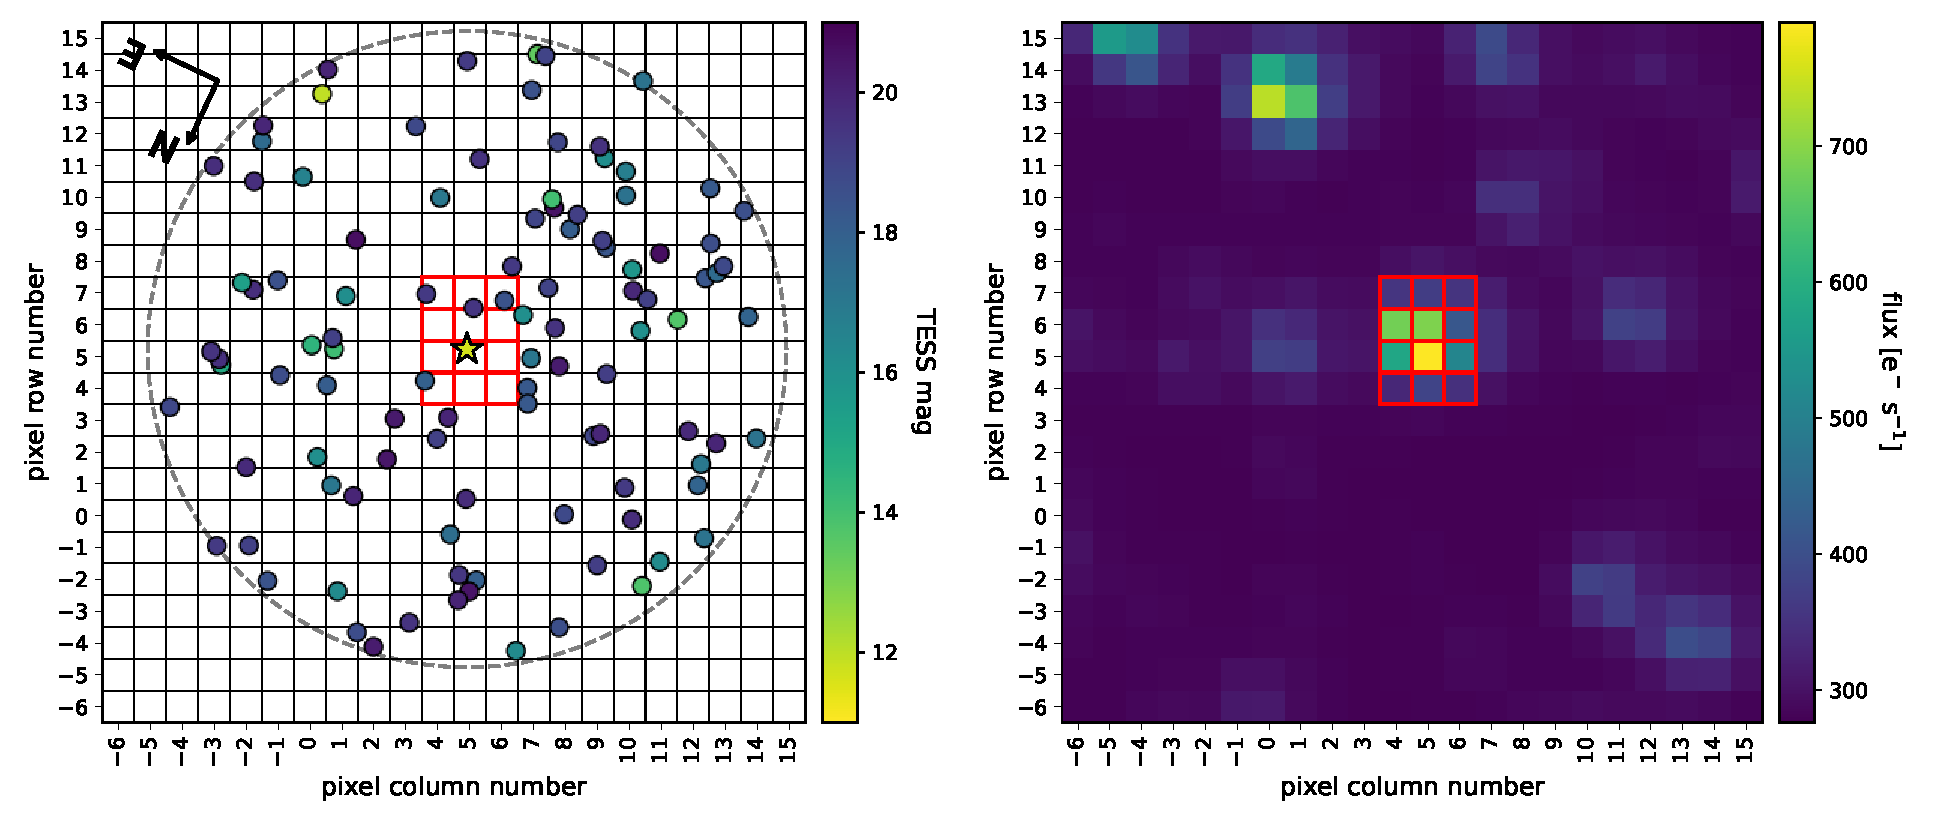
\includegraphics[width=0.8\textwidth]{l27994_field_s94.pdf}
\caption{Sector 94: TIC stars on the TESS pixel grid (left) and the image
with the optimal aperture (right). L~279-94 dominates its aperture.}
\label{fig:l279-field}
\end{figure}

\section*{Results}

\begin{longtable}{@{}p{0.38\textwidth}p{0.55\textwidth}@{}}
\toprule
\textbf{Quantity} & \textbf{Result}\\
\midrule\endhead
Star (TIC) & $T_\mathrm{eff} = 3491$~K, $R = 0.41~R_\odot$, $M = 0.40~M_\odot$\\
Transits & 7 in 5 sectors (one more than published; the one at the start
of sector 104 is weak, S/N 3)\\
Ephemeris & P = 18.15222~d, T0 = BTJD 2036.9718 (refined from the 7 transits)\\
Depth & 3690~ppm (limb-darkened fit), 3510~ppm on the target\\
Duration, shape & T14 = 2.36~h, U-shaped, not grazing; $R_p/R_\star = 0.057$\\
Planet radius & 2.5--2.8~$R_\oplus$: a sub-Neptune\\
Depth consistency & $\chi^2_\nu = 0.9$ over the 7 transits; odd/even 0.8$\sigma$\\
Secondary eclipse & none; 3$\sigma$ limit 525~ppm (a companion would be cooler than 2540~K)\\
Timing (ETV) & O$-$C rms 6.9~min, no significant trend\\
Stellar density & 11.9~g\,cm$^{-3}$ from the transit at $b = 0.32$, 8.2 from the TIC; $b$ is unconstrained ($\pm1.6$), so no conflict\\
Neighbours & the star at 41$''$ named in the Zenodo note (TIC~100795619)
is excluded by the difference imaging (6--8$\sigma$ from the centroid in
sectors 67 and 105); no other neighbour can produce the dip (NFPP = 0)\\
Difference imaging & centroid on the target (median 0.4$\sigma$, 3 of 5 sectors with enough S/N in v4.3)\\
FPP / NFPP, default companions & 0.036 $\pm$ 0.005 (10-min bins, three runs), 0.032 $\pm$ 0.004 (5-min bins) / 0\\
FPP / NFPP, Gaia-limited companions & 0.0070 $\pm$ 0.0015 / 0 (MOLUSC, 10-min bins)\\
Verdict & NOT passed with the default companion prior; PASSED with the companions Gaia still allows, under the assumption discussed below\\
\bottomrule
\end{longtable}

\begin{figure}[ht]
\centering
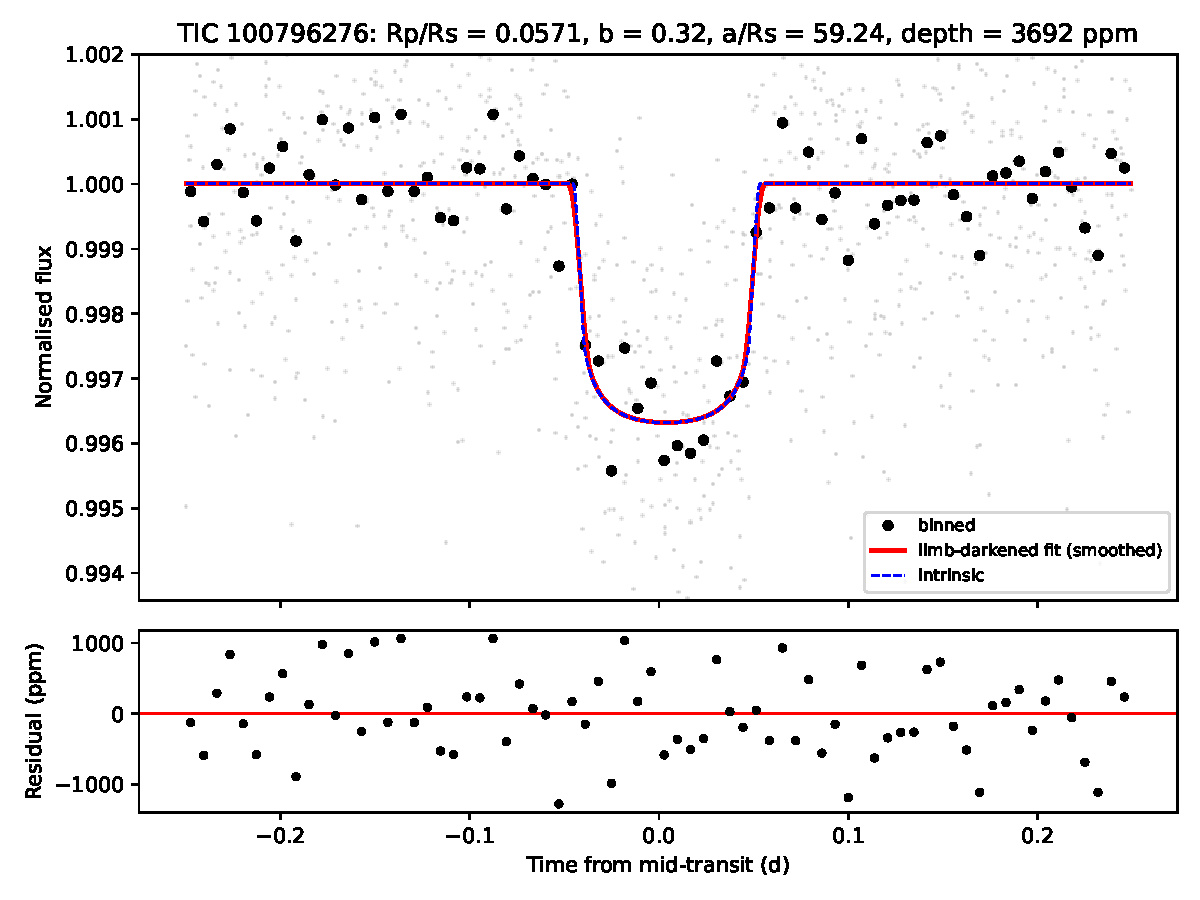
\includegraphics[width=0.49\textwidth]{l27994_ld_fit.pdf}\hfill
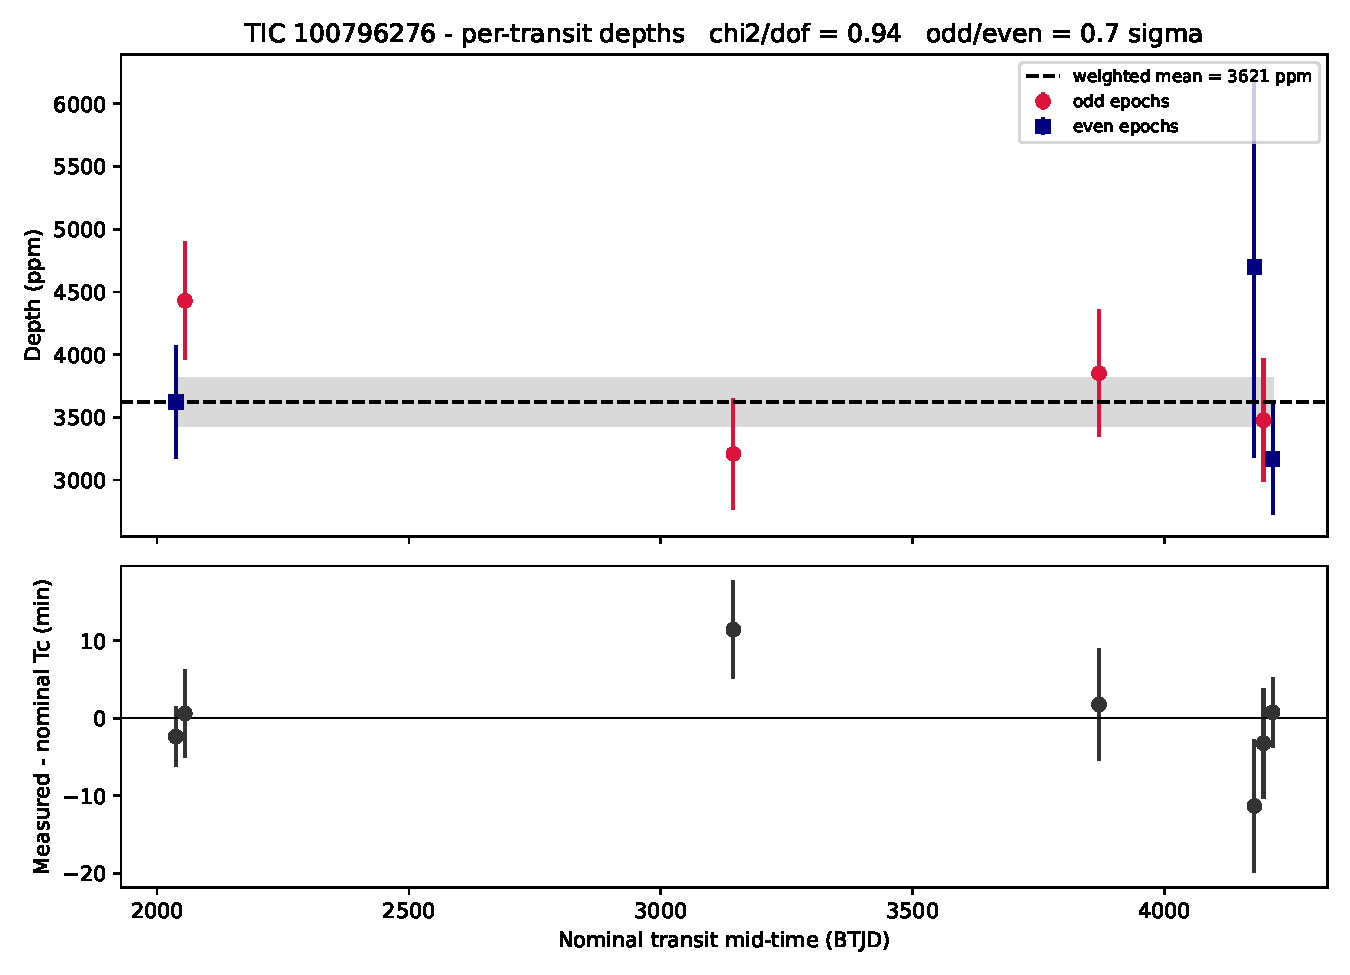
\includegraphics[width=0.49\textwidth]{l27994_per_transit.pdf}
\caption{Left: the seven transits folded, with the limb-darkened fit
(10-min bins). Right: depth and mid-time of each transit; odd (red) and even
(blue) agree.}
\label{fig:l279-fit}
\end{figure}

\section*{Comparison with the Zenodo note}

The two analyses are independent (other light curves, other code) and
agree on everything the light curve measures:

\begin{center}
\begin{tabular}{@{}p{0.27\textwidth}p{0.34\textwidth}p{0.32\textwidth}@{}}
\toprule
 & Rabtsevich (2026) & This pipeline\\
\midrule
Period & 18.15219 $\pm$ 0.00003~d & 18.15222~d\\
Depth, duration & 0.32~\%, 2.4~h & 0.35--0.37~\%, 2.36~h\\
Planet radius & 2.54 $\pm$ 0.10~$R_\oplus$ & 2.5--2.8~$R_\oplus$\\
Insolation & 2.4 $\times$ Earth & 2.3 $\times$ Earth\\
Transits & 6 (the 7th, at the start of sector 104 in stray light, left out) & 7 (the 7th weak, S/N 3)\\
Source of the dip & within $\sim$5$''$ of the star; TIC~100795619 very unlikely & centroid on the target; TIC~100795619 excluded\\
Secondary eclipse & none ($<$0.05--0.07~\%) & none ($<$0.05~\%)\\
FPP, default companions & 0.022 (TRICERATOPS 1.1.0) & 0.037 (TRICERATOPS+ 1.0.17)\\
FPP, companions limited by Gaia (MOLUSC) & 0.003--0.004 (passes) to 0.042 & 0.0070 $\pm$ 0.0015 (passes, 10-min bins)\\
\bottomrule
\end{tabular}
\end{center}

The note gives seven TRICERATOPS results under different assumptions. With
the default companion prior both analyses stay above the bar of 0.015. With
the companions that Gaia still allows (computed with MOLUSC, Wood et al.\
2021) the note's main analysis passes, but not with every treatment of the
data (10-min bins fail), and its second analysis fails. Two of its remarks
matter for this pipeline: the ingress of this planet lasts about 11~min,
so 10-min bins blur the shape of the transit; and TRICERATOPS 1.1.0 ignores
companions closer than about 3~au, the version used here does not, which
alone makes our FPP higher.

We therefore repeated the run with 5-min bins (\code{--bin-minutes 5},
profile \code{profile_TIC100796276_bin5}). The FPP changes from 0.036 to
0.032, within the run-to-run scatter: with the default companion prior the
bin width does not matter for this star. Two side effects of the shorter
bins taught us something. The free limb-darkened fit, now with more noise
per bin, jumped to a long, grazing solution ($b = 0.91$, T14 = 3.1~h)
that implies a stellar density of 0.9~g\,cm$^{-3}$, impossible for an M
dwarf of 0.4~$M_\odot$; since v4.3 such a fit is repeated with a prior on
the catalogue density (here: $b = 0.48$, T14 = 2.40~h). And the depth check
before TRICERATOPS used the three lowest bins of the fold, which noise makes
too deep; it now uses the median of the central bins. The note concludes,
as we do, that the candidate is not validated.

\section*{Why it is not validated}

Every test the light curve allows is passed. What remains is one scenario
that TESS cannot test: \textbf{STP}, the same planet transiting an
unresolved \emph{bound companion} of similar mass (best fit 0.36~$M_\odot$,
45~\% of the light). The probabilities of the last TRICERATOPS iteration are

\begin{center}
\begin{tabular}{@{}lll@{}}
\toprule
Planet on the target & TP 0.82, PTP 0.10, DTP 0.05 & 0.97\\
Planet on a bound companion & STP & 0.033\\
All eclipsing-binary scenarios & & $< 0.001$\\
\bottomrule
\end{tabular}
\end{center}

STP is a false positive in the sense of TRICERATOPS (the planet would not
orbit the target, and it would be larger, about 3.8~$R_\oplus$), and its
probability comes almost entirely from the \emph{prior}: M dwarfs often have
companions, and a twin companion leaves the light curve unchanged. This
also explains the sensitivity test:

\begin{center}
\begin{tabular}{@{}lcccc@{}}
\toprule
Noise $\times$ & 0.5 & 1 & 2 & 4\\
FPP, 6 Nov (v4.1.1) & 0.010 & 0.036 & 0.032 & 0.042\\
FPP, 19 Nov, run A (v4.3) & 0.055 & 0.037 & 0.033 & 0.043\\
FPP, 19 Nov, run B (v4.3) & 0.005 & 0.034 & 0.031 & 0.043\\
FPP, 20 Nov, 5-min bins (v4.3) & 0.559 & 0.034 & 0.030 & 0.042\\
\bottomrule
\end{tabular}
\end{center}

The FPP hardly depends on the assumed noise: it is set by the companion
prior, not by the quality of the light curve. Only the optimistic case
(half the measured noise) sometimes passes, which the audit flags as
\emph{not a validation}. The two identical runs of 19~November show why
that case cannot be trusted anyway: at half the noise the likelihoods are
sharper, the Monte-Carlo sampling noisier, and three pooled runs give 0.055
in one run and 0.005 in the other; with 5-min bins the same case even gives
0.56, because half the measured noise is then well below the white noise of
a bin (470 against 760~ppm) and no model fits. The nominal FPP, from 20 runs, is
reproducible to $\pm0.003$. More TESS data will not change this; an observation that
looks for companions will. The Zenodo note reaches the same point from the
other side: its FPP drops below 0.015 only when Gaia is used to limit the
companions.

\section*{With the companions Gaia still allows (MOLUSC)}

MOLUSC (Section~\ref{sec:molusc}) simulated $10^6$ possible companions of
L~279-94 and compared each with the Gaia DR3 astrometry (RUWE = 1.32) and
Gaia imaging (profile \code{profile_TIC100796276_molusc}, script
\code{MOLUSC/run_molusc_L27994.sh}). The survivors, by closest approach
to the star:

\begin{center}
\begin{tabular}{@{}lrrl@{}}
\toprule
Periastron & Survivors & of which $q > 0.75$ & used by TRICERATOPS\\
\midrule
$<$ 1~au & 205\,995 & 45\,578 & no\\
1--3~au & 58\,886 & 7\,760 & no\\
3--10~au & 47\,767 & 1\,704 & no\\
10--100~au & 85\,266 & 3\,852 & yes\\
$>$ 100~au & 67\,569 & 654 & yes\\
\midrule
All & 465\,483 (46.5~\%) & 59\,548 & 152\,835 (15.3~\%)\\
\bottomrule
\end{tabular}
\end{center}

Gaia excludes more than half of all companions. Beyond 10~au few
\emph{bright} ones remain (mass ratio $q > 0.75$, the near-twins that STP
needs): 4\,506 per million, against 45\,578 within 1~au. With these companions, and every star assumed to have one,
TRICERATOPS gives

\begin{center}
\begin{tabular}{@{}lcc@{}}
\toprule
 & default companions & Gaia-limited (MOLUSC)\\
\midrule
TP / PTP / DTP & 0.82 / 0.11 / 0.05 & 0.81 / 0.13 / 0.05\\
STP & 0.025--0.033 & 0.006\\
FPP (pooled, 20 runs) & 0.032--0.037 & 0.0070 $\pm$ 0.0015\\
FPP at 0.5 / 2 / 4 $\times$ the noise & 0.005--0.56 / 0.03 / 0.04 & 0.000 / 0.007 / 0.015\\
Verdict & NOT passed & PASSED\\
\bottomrule
\end{tabular}
\end{center}

and the audit has no FAIL (one WARN, the unconstrained impact parameter);
its \emph{Evaluation} names the companion prior. This agrees with the main
analysis of the Zenodo note (0.003--0.004).

\textbf{What the pass rests on.} The table shows the catch. Most surviving
near-twin companions (45\,578 of 59\,548) come closer than 1~au to the
star: Gaia cannot see them, and with no radial velocities nothing rules
them out. They do not count because TRICERATOPS uses only companions
beyond 10~au, on the grounds that planets are rare in close binaries. For
an 18-day planet at 0.1~au a companion within $\sim$0.4~au would make the
orbit unstable anyway, but between about 0.4 and 10~au planets are
suppressed, not forbidden. The Zenodo note's second analysis, which keeps
these companions, does not pass (FPP 0.030). The honest summary is
therefore: \emph{L~279-94~b passes the validation criteria when Gaia limits
the wide companions and planets are assumed absent in binaries closer than
10~au}. Spectroscopy, which sees exactly those close companions, would turn
the assumption into a measurement.

\section*{Is it in the habitable zone?}

The Zenodo note does not claim it is; it gives the insolation (2.4 times
the Earth's). The question comes up whenever a planet orbits an M dwarf, so
here is the comparison.


With the TIC parameters the star emits 2.3~\% of the Sun's luminosity and
the planet orbits at 0.100~au. It receives
$S = 2.3 \pm 0.5$ times the insolation of the Earth (more than Venus,
1.9), and its equilibrium temperature is 310--340~K (Bond albedo 0.3--0).
The habitable zone of this star (Kopparapu et al.\ 2014) begins at
$S = 1.5$ (optimistic inner edge, ``recent Venus'', P $\approx$ 25~d) and
the conservative zone lies between $S = 0.93$ and 0.25 (P = 35--96~d)
(Figure~\ref{fig:l279-hz}). The candidate is therefore a \emph{warm
sub-Neptune just inside the inner edge}, not a habitable-zone planet; and at
2.5--2.8~$R_\oplus$ it is most likely not rocky. A planet further out in
the same system could lie in the zone: 25--96~d periods are well within
reach of TESS and of ground photometry.

\begin{figure}[ht]
\centering
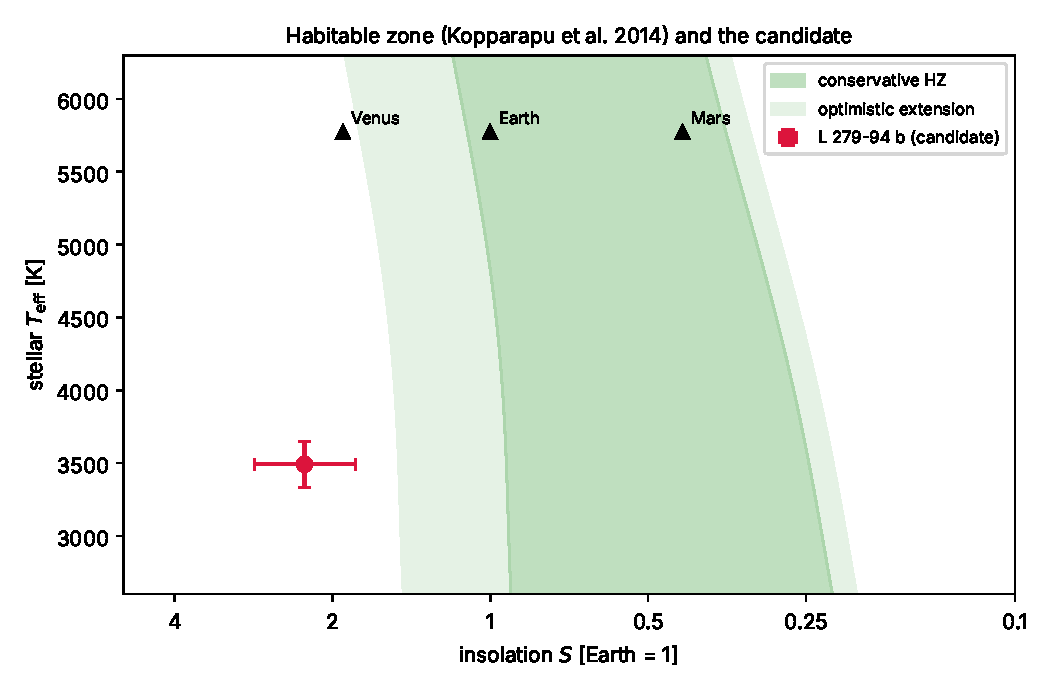
\includegraphics[width=0.7\textwidth]{l27994_hz.pdf}
\caption{Insolation of the candidate (red; error bar from the TIC
uncertainties of $T_\mathrm{eff}$ and radius) against the habitable zone
for main-sequence stars. Dark green: conservative zone (runaway to maximum
greenhouse); light green: optimistic extensions (recent Venus, early Mars).
Venus, Earth and Mars for comparison.}
\label{fig:l279-hz}
\end{figure}

\section*{What observers can do}

With the default companion prior the audit page \emph{Next observations}
ranks three observations, all aimed at the STP scenario. With MOLUSC the
criteria are already met; the same observations then test its assumptions,
and spectroscopy moves to the first place because it sees the close
companions that Gaia cannot:

\begin{enumerate}
\item \textbf{Transits in two bands} ($g'$ and $z'$, simultaneous if
possible). A planet on L~279-94 gives the same depth in both. On the
best-fit companion (about 3140~K, cooler than the target) the depth in $g'$
would be only 0.77 times that in $z'$: about 930~ppm apart, visible at
3$\sigma$ with a depth error of $\leq$310~ppm per band. The audit estimates
that a typical result brings the FPP to 0.007 --- enough on its own.
Several transits per band can be combined; TRICERATOPS+ uses them directly
(Section~\ref{sec:multiband}), and the audit's \emph{Multi-band} test then
states which scenarios they exclude.
\item \textbf{High-resolution imaging} (speckle, adaptive optics): at
43.5~pc, 0.1$''$ is 4.4~au, so most bound companions would be resolved.
Typical outcome FPP 0.017; give the contrast curve to the pipeline with
\code{--contrast-curve}.
\item \textbf{Reconnaissance spectroscopy}: a companion with 45~\% of the
light shows a second set of lines. Typical outcome FPP 0.011.
\end{enumerate}

According to the Zenodo note, Gaia DR4 (scheduled for 2~December 2026)
will add five and a half years of astrometry, which can reveal companions
directly; MOLUSC should then be rerun with the
new values.

\textbf{Practical.} The transit is 3.5~ppt deep and lasts 2.4~h; with
$V = 13.9$ but $T \approx I \approx 11.7$ the star is much brighter in the red, so
$z'$ (or I) gives the best precision and $g'$ (or V) is the demanding band.
At declination $-53^\circ$ it is a southern-hemisphere target, best
observed from June to September. Predicted mid-transits (formal error
$\pm7$~min; observe at least 1~h before and after):

\begin{center}
\begin{tabular}{@{}lll@{}}
\toprule
Mid-transit (BJD\_TDB) & UTC (approx.) & Night side\\
\midrule
2461560.131 & 2027 June 3, 15:07 & Australia\\
2461578.283 & 2027 June 21, 18:47 & Australia (morning)\\
2461596.435 & 2027 July 9, 22:26 & South Africa\\
2461614.587 & 2027 July 28, 02:05 & South America, South Africa\\
2461632.739 & 2027 August 15, 05:44 & South America\\
2461669.044 & 2027 September 20, 13:03 & Australia\\
\bottomrule
\end{tabular}
\end{center}

The GUI tool \emph{Predicted transit times} gives the times for any
date range (Section~\ref{sec:tools}). The Zenodo note predicts the
transits of 4 and 22~December 2026 at 02:40 and 06:20~UTC ($\pm3$~min);
our ephemeris gives 02:35 and 06:15 ($\pm7$~min): consistent.

\begin{tip}
\textbf{Lessons.}
(1)~A clean light curve is not a validation: when every test passes and
the FPP stays at a few per cent, look at \emph{which} scenario holds it.
(2)~If the FPP barely changes with the assumed noise, it is set by a prior
(here: bound companions of M dwarfs), and only an observation that tests
that prior can lower it.
(3)~``Habitable zone'' needs a number: compute the insolation from the
stellar luminosity and the orbit, and compare with the zone of a star of
that temperature.
(4)~The FPP of a candidate like this depends on modelling choices
(companion prior, bin width, TRICERATOPS version): report it with the
choices, as the Zenodo note does, and test the obvious alternatives
(\code{--bin-minutes 5}, \code{--molusc-file}).
(5)~Repeat a run before trusting a number that sits near a threshold: two
identical runs are the cheapest test of Monte-Carlo noise
(\code{--sens-runs} raises the number of runs per sensitivity case).
(6)~Gaia (through MOLUSC) can turn a ``not validated'' into ``validated''
without telescope time, but only for the companions Gaia could have seen;
state the companion model and what it assumes about close binaries.
\end{tip}
